\documentclass[12pt,a4paper]{ctexart}
\usepackage{geometry}
\usepackage{booktabs}
\usepackage{graphicx}
\usepackage{float}
\usepackage{amsmath}
\geometry{margin=2.5cm}

\title{基于初级分类的行业异质性分析（探索版）}
\author{}
\date{\today}

\begin{document}
\maketitle

\section*{一、行业差距}

\subsection*{1. Entropy/HHI 的行业差距}
本节基于岗位级 Global LDA 指标（Entropy 与 HHI）进行初级分类异质性比较。样本期为 2016--2025 年，且在年度分类统计中仅将样本量 $sample\_n \ge 500$ 的单元格记为有效点。

\paragraph{探索性异质性分析：方法一：Entropy）}
方法一仅使用 Entropy 指标。具体做法是：先按 ``年份 $\times$ 初级分类'' 计算平均 Entropy，再绘制多行业时间折线。横轴为年份，纵轴为 Entropy，不同颜色代表不同行业（C1--C8）。

\begin{figure}[H]
    \centering
    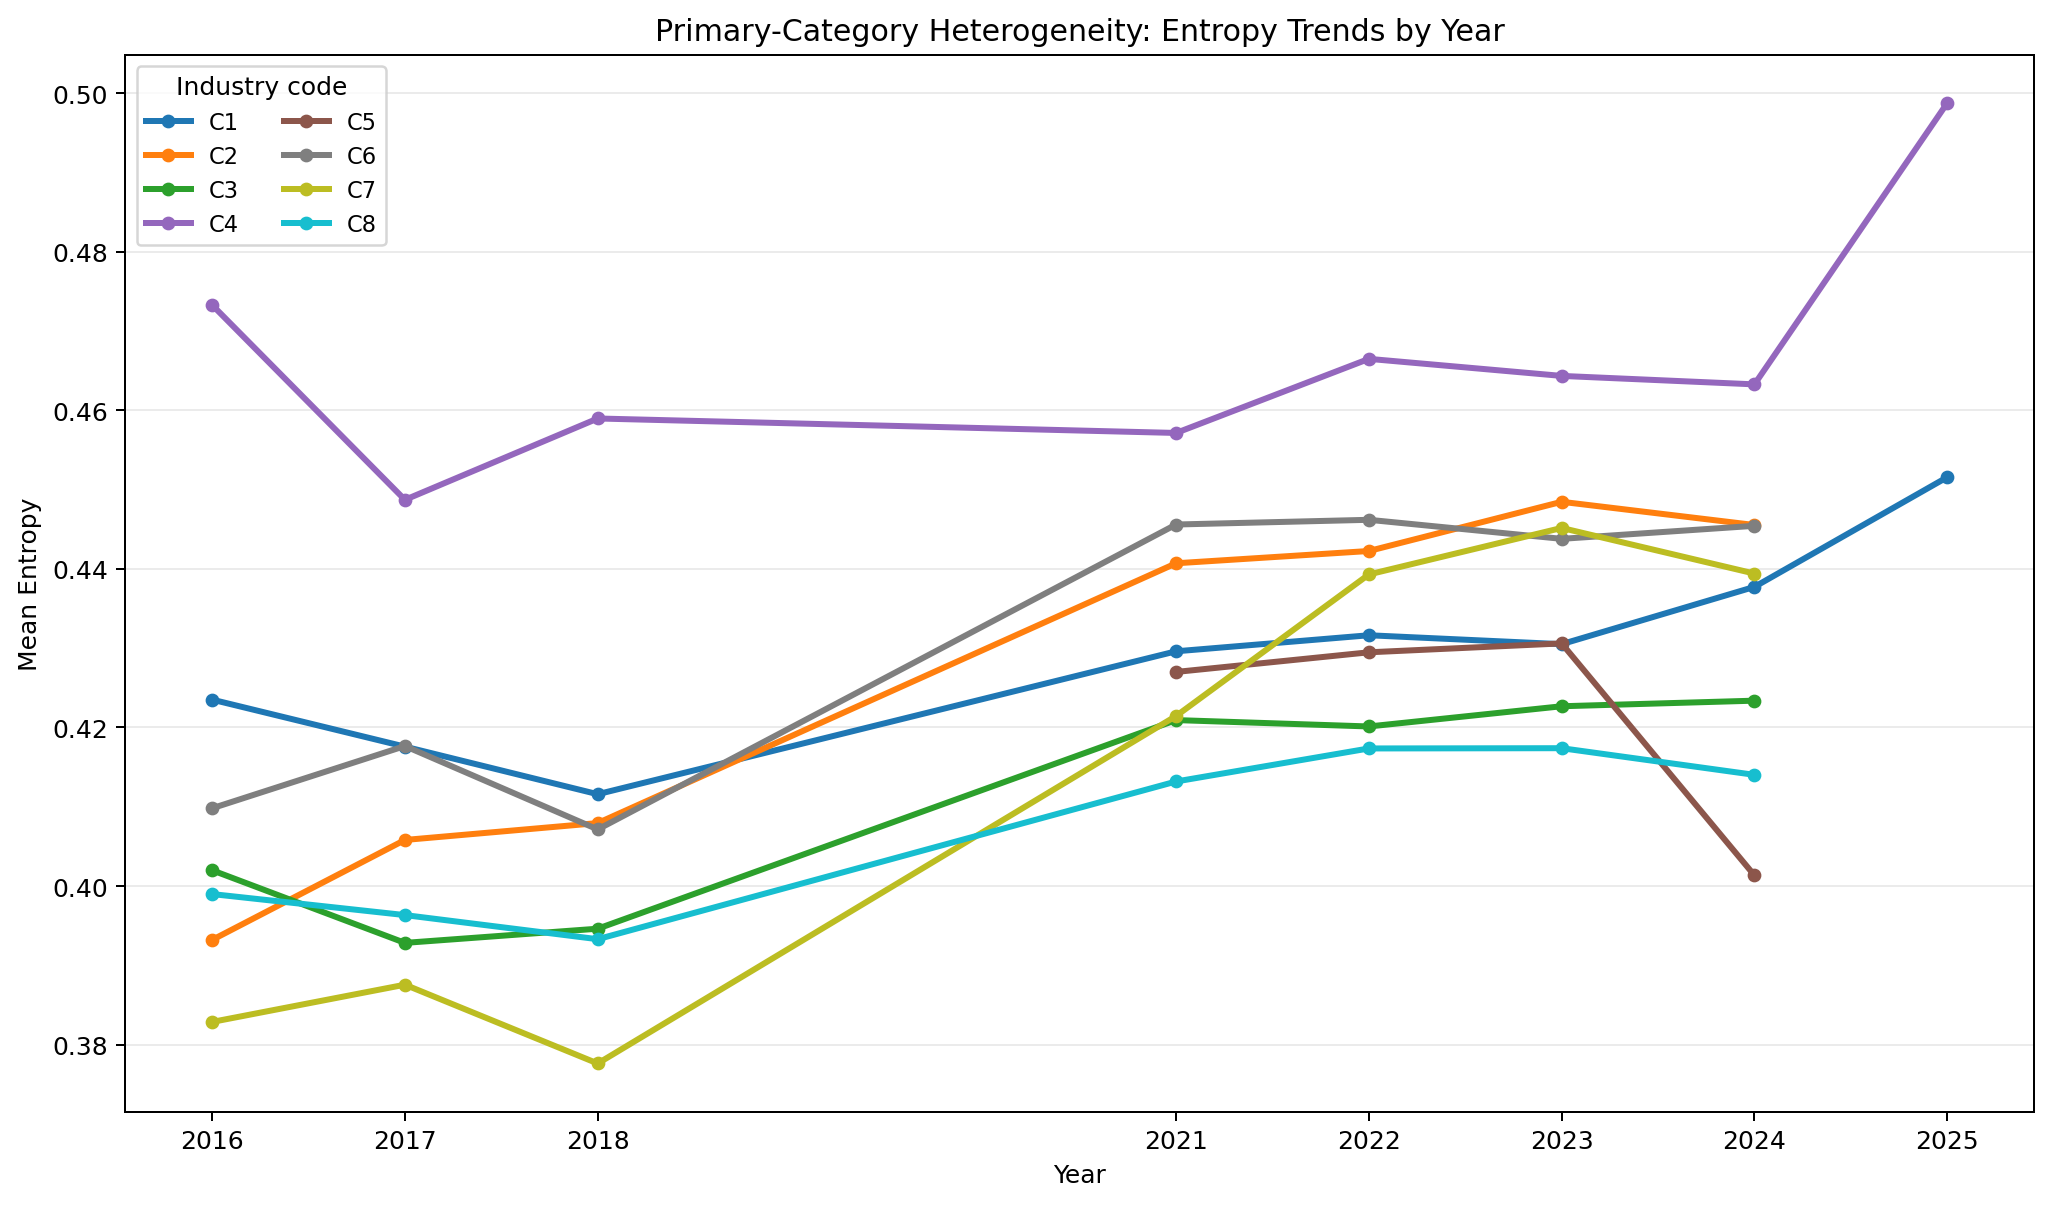
\includegraphics[width=0.95\textwidth]{figures/primary_category_entropy_only_lines.png}
    \caption{探索性异质性方法一：Entropy 多行业年度折线图（颜色区分行业）}
\end{figure}

图中 C1--C8 对应高样本初级分类（见后文代码表），可直接比较不同行业在 2016--2025 年综合化程度的演进斜率与波动幅度。

\paragraph{横截面差距（以 2024 年为例）}
在 2024 年且 $sample\_n \ge 2000$ 的 89 个初级分类中，平均 Entropy 的区间为 $[0.361,\ 0.495]$，存在明显分类差距。高 Entropy 分类包括 ``检测/认证''（0.495）、``旅游服务''（0.481）；低 Entropy 分类包括 ``房地产中介''（0.361）、``人力资源服务''（0.401）。

\paragraph{时间变化差距（2016 $\rightarrow$ 2024）}
在同时满足 2016 与 2024 年有效样本条件的 24 个初级分类中，多数分类 Entropy 呈上升，且 HHI 同步下降。提升较快的分类包括 ``计算机软件''（$\Delta Entropy=+0.0565$）、``互联网''（$+0.0523$）、``IT服务''（$+0.0526$）；而 ``咨询服务'' 出现小幅回落（$-0.0100$）。

\subsection*{2. 技能结构变迁}
本节统一采用主文档中同一套 Window LDA + Alignment 口径。结构变迁由相邻窗口的事件率衡量：
\begin{itemize}
    \item \textbf{存活率（Survival Rate）}：上一窗口主题在下一窗口找到一对一延续映射的比例；
    \item \textbf{重组率（Reorganization Rate）}：$1-\text{存活率}$，包含分裂（Split）与融合（Merge）事件。
\end{itemize}

更关键的是，alignment 在本节按\textbf{不同行业（初级分类）}展开：对每个窗口迁移，统计该行业中落在 ``存活主题'' 上的岗位占比，得到行业技能存活率。为保证稳健性，仅保留源窗口样本量 $n\_{\text{source}}\ge 500$ 的行业-窗口单元。

在高样本 8 个初级分类中，平均技能存活率约在 61.7\%--70.0\% 区间。整体上，``房地产开发'' 与 ``医药制造'' 的存活率相对较高；``快速消费品'' 相对较低。该差异说明：即使在同一宏观时期，不同行业的技能边界稳定性和重组强度也并不同步。

\begin{figure}[H]
    \centering
    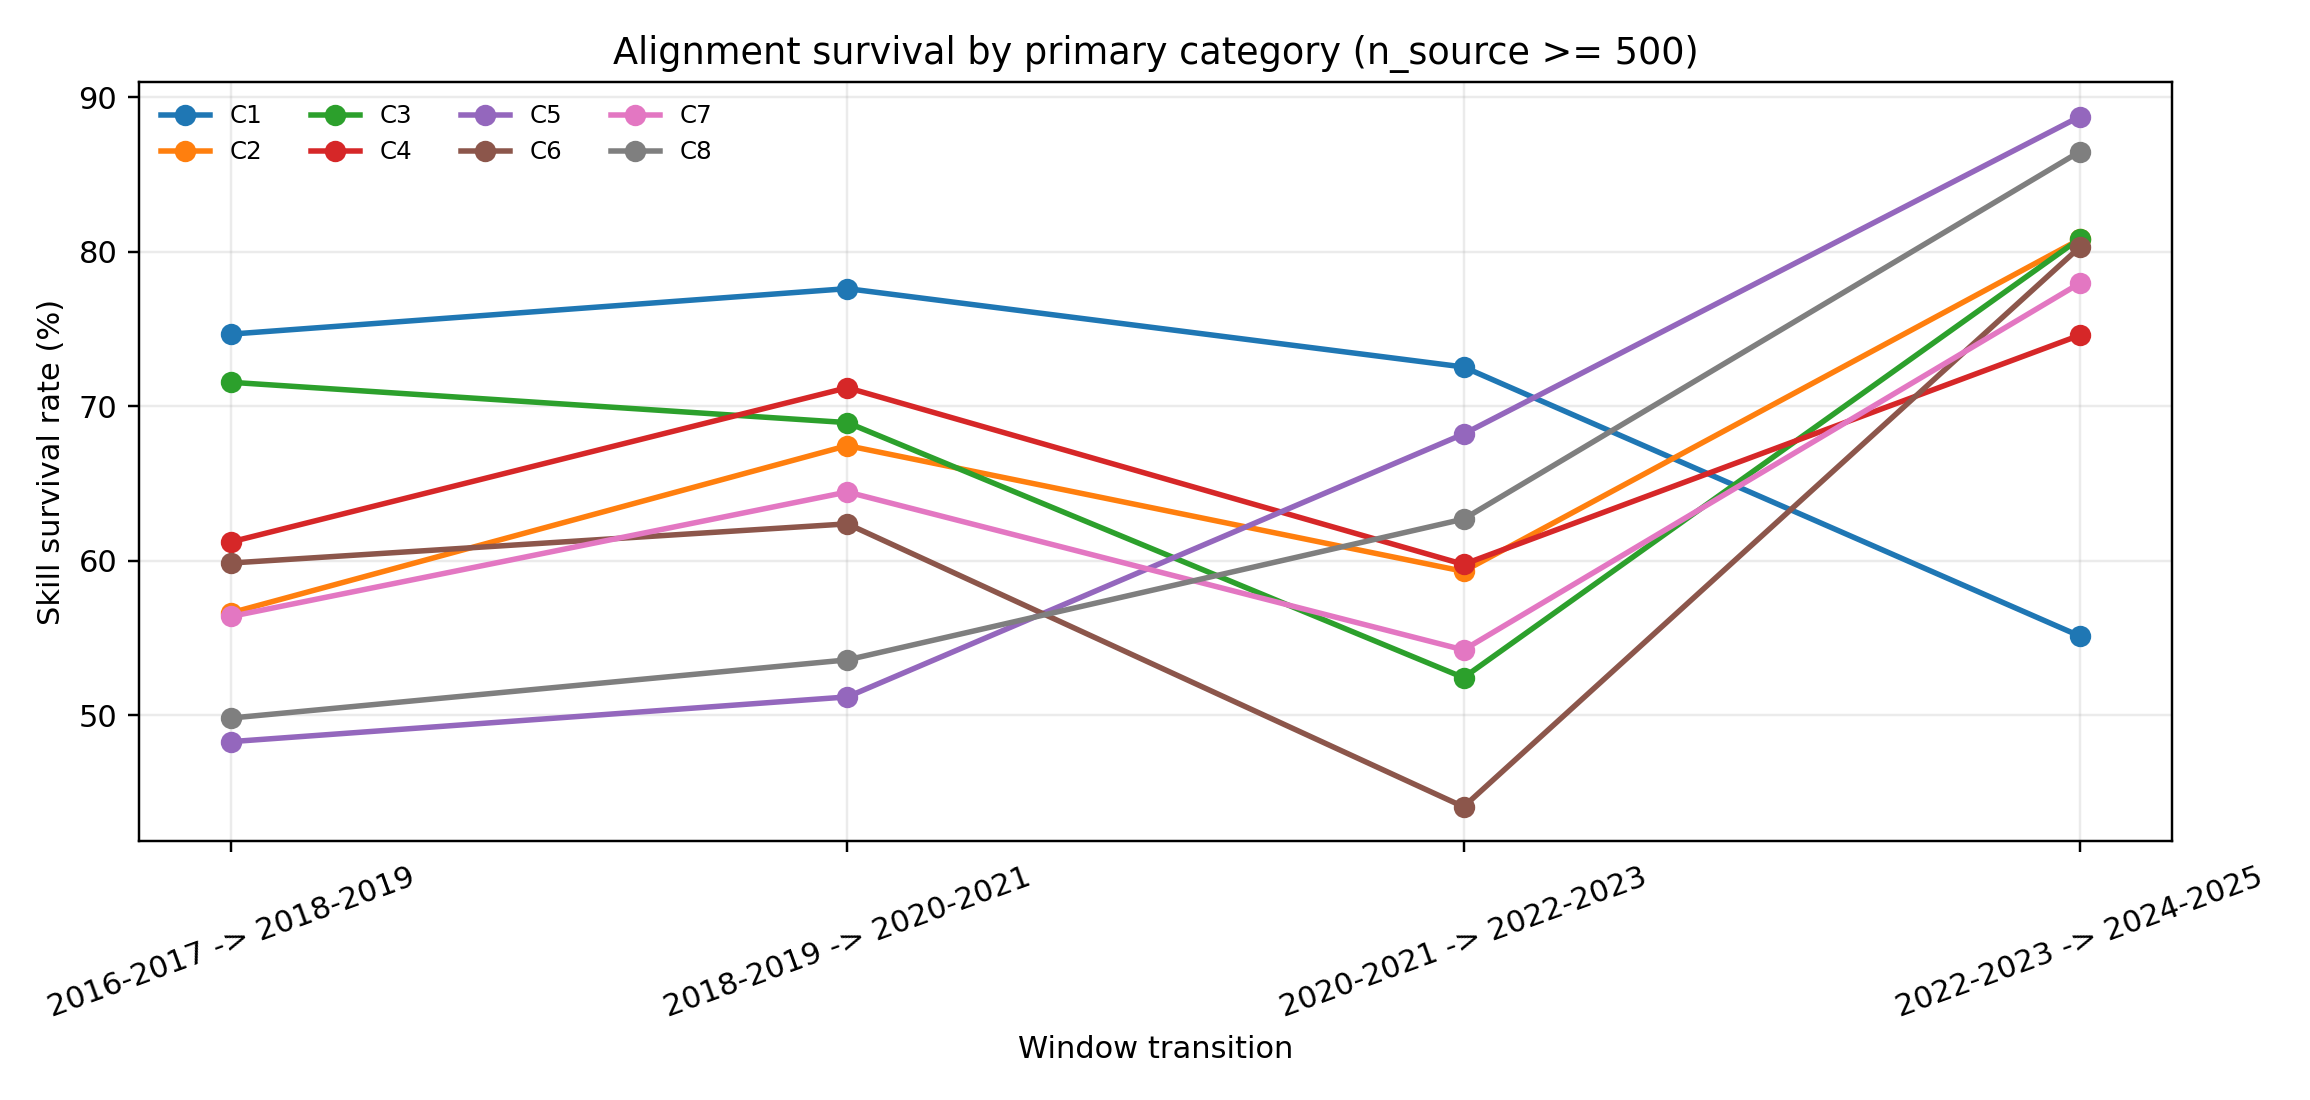
\includegraphics[width=0.95\textwidth]{figures/primary_category_alignment_survival.png}
    \caption{Alignment 口径下的不同行业技能存活率（初级分类，$n\_{\text{source}}\ge 500$）}
\end{figure}

\begin{table}[H]
\centering
\caption{图中分类代码说明}
\begin{tabular}{ll}
\toprule
代码 & 初级分类 \\
\midrule
C1 & 房地产开发 \\
C2 & 互联网 \\
C3 & 医药制造 \\
C4 & 咨询服务 \\
C5 & 人力资源服务 \\
C6 & 电子/半导体/集成电路 \\
C7 & 计算机软件 \\
C8 & 快速消费品 \\
\bottomrule
\end{tabular}
\end{table}

\section*{二、数据说明}

\subsection*{1. 初级分类口径并非统一标准}
``初级分类'' 来自原始招聘数据字段，来源平台与填报实践并不完全一致，存在同义并存、粒度不一致、跨域混用等问题。因此，本分析更适合作为 \textbf{探索性异质性分析}，不宜直接作为最终行业口径。

\subsection*{2. 缺失值比例较高}
在当前主表（7,768,501 条岗位记录）中，``初级分类'' 非空覆盖率约为 47.98\%，对应缺失率约 52.02\%。这会导致两类偏差风险：一是样本选择偏差，二是部分分类在末期（如 2025 年）有效样本不足。

\subsection*{3. 下一步：映射到 20 个经济活动门类}
基于上述限制，下一步将采用 ``公司名称 + 岗位名称'' 的联合映射方案，将岗位映射到国民经济活动 20 个门类（A--T）并重算异质性指标。该方案目标是提升口径一致性与跨期可比性，作为正式实证口径。

\end{document}
